\documentclass{article}

%%%%%%%%PACKAGES%%%%%%%%
\usepackage{amsmath} 
\usepackage{amsfonts}
\usepackage{siunitx} 
\usepackage{physics}
\usepackage{geometry}
\usepackage{graphicx}
\usepackage{float}
\geometry{margin=1in} 

%%%%%%%%TITLE%%%%%%%%
\title{Notes on Higher-Form Symmetries}
\author{Gabriel C. Magalhães\footnote{gabriel.capelini@uel.br}}
\date{2025}

\begin{document}
\maketitle

\section*{Introduction}
Higher-form symmetries are the straight generalization of our “usual” notion of symmetries. It consists in assigning a topological meaning to symmetry operators and extending the parameter of the transformation to extended objects such as lines, surfaces and so on. Below we rephrase our notion of symmetries in terms of topological operators in a way that we can generalize it. 

\section*{Symmetry Operators as Topological Operators}
We’ve saw that in terms of differential forms, the conservation law is written as
\begin{equation*}
	d\star j=0,
\end{equation*}
where $j$ is the current 1-form and $\star:\Lambda^p\to \Lambda^{D-p}$   is the Hodge star map that take a p-form and associates it to a $(D-p)$-form. Thus the conserved charge was defined as
\begin{equation*}
	Q\equiv\int d^{D-1}x\;j^0.
\end{equation*}
In terms of differential forms, we may write as
$$
Q=\int_{\Sigma_{D-1}}\star j,
$$
where $\Sigma_{D-1}$  is a $D-1$  manifold. We say then that those charges are integrated over a manifold of codimension 1, which is a submanifold of a manifold of dimension $D$.  To understand how these operators act over the fields, we will make use of the Ward identity,
$$
\partial_\mu\langle j^\mu(x)\phi(y)\rangle=-i\delta^{(D)}(x-y)\langle\delta\phi(y)\rangle.
$$
Integrating over a D-dimensional manifold $\Omega$  with boundary $\Sigma_{D-1}$, the left-hand side becomes
$$
\int_{\Omega}d\langle\star j\phi(y)\rangle=\int_{\Sigma_{D-1}}\langle\star j\phi(y)\rangle=\langle Q(\Sigma_{D-1})\phi(y)\rangle,
$$
where we used Stokes theorem. For the right-hand side, we have
$$
-i\int_{\Omega}d^Dx\;\delta^{(D)}(x-y)\langle\delta\phi(y)\rangle,
$$
where we identify,
$$
\int_{\Omega}d^Dx\;\delta^{(D)}(x-y)=\begin{cases}0,\quad y\in\Omega\\1,\quad y\not\in\Omega\end{cases}
$$
as the linking between the point $y$ and the manifold $\Omega$. Thus we call  
$$
\int_{\Omega}d^Dx\;\delta^{(D)}(x-y)\equiv \text{Link}(\Sigma_{D-1},y).
$$
Hence
$$
\langle Q(\Sigma_{D-1})\phi(y)\rangle=-i\text{Link}(\Sigma_{D-1},y)\langle\delta\phi(y)\rangle.
$$
What this expression is telling us is that the charge acts on the local field and it only have non-vanishing action if the point where the local operator is defined links with the manifold in which the charge is defined. The link is unaffected by deformations as longs as they do not cross the point $y$.  To see why, suppose that we perform a deformation of the type $\Sigma'=\Sigma+\Sigma_0$, $y\not\in\Omega_0.$ Then 
$$
Q(\Sigma+\partial\Omega_0)=\int_{\Omega\cup\Omega_0}\langle d\star j\phi(y)\rangle=\int_{\Omega}\langle d\star j\phi(y)\rangle+\int_{\Sigma_0}\langle d\star j\phi(y)\rangle.
$$
Since $\text{Link}(\Sigma_0,y)=0,$ then
$$
Q(\Sigma+\partial\Omega_0)=\int_{\Omega}\langle d\star j\phi(y)\rangle=Q(\Sigma).
$$
This is why we call these \textit{topological operators}. The unitary operator is defined by taking the exponential of the conserved charge,
$$
U(g,\Sigma_{D-1})=\exp(i\alpha_aQ_a)=\exp\left(i\alpha\int\star j\right),
$$
where $g\in G$  is an element of the group $G$ and $\alpha_a$ are the parameters of the transformation. In the case of  $U(1)$  we have $g=e^{i\alpha}$.  We say then that this is a *topological codimension-1 operator. 

We may understand the the action of 0-form symmetries in terms of the unitary operators as well. Recall that the local operators transform under some transformation by
$$
U_g(t)\mathcal{O}(x)U^{-1}_g(t)=\mathcal{O}'(x).
$$
Where these operators are defined in some spatial slice $\Sigma_{D-1}$. The corresponding expression for topological operators is given by 
$$
\langle U(\Sigma_{D-1})\mathcal{O}(x)\rangle=\langle \mathcal{O}'(x)U(\Sigma'_{D-1})\rangle.
$$
Since operators are defined over a Hilbert space at a constant time, we can not compare operators at different times. Since the manifold $\Sigma_{D-1}$ need not to be necessarily a spatial slice for general topological operators, the expression only makes sense inside correlation functions, where we can compare operators at different spacetime points without problem. Thus we assume that $\Sigma'_{D-1}$ is a slice at a different time, say $t'$. Note that taking the limit $t\to t'$ we recover the usual transformation law. What is happening diagrammatically is shown below. 

Let   $U(S^{D-1})$ be an operator defined over a $(D-1)$-sphere.  As we have seen, these operators act over local operators $\mathcal{O}(x)$ and transforms them into another operator $\mathcal{O}'(x)$  as shown in the figure
\begin{figure}[h]
\centering
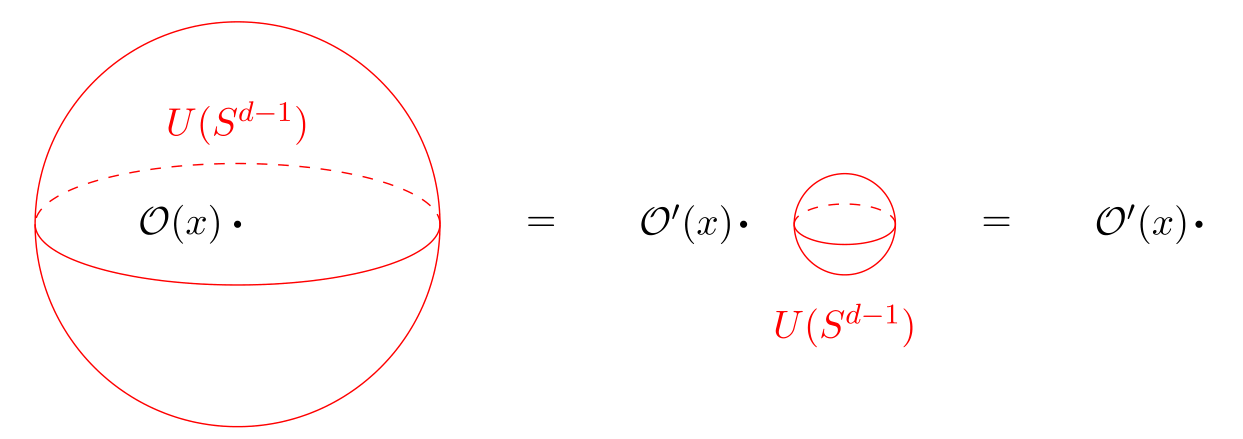
\includegraphics[scale=0.4]{figures/linking.png}
\caption{Taken from Bhardwaj}
\end{figure}
he operator $U(S^{D-1})$ links with $\mathcal{O}(x)$ then we deform it until it no longer links. Then we can deform the $S^{D-1}$ to a point and the reminiscent operator is what we call $\mathcal{O}'(x).$ The mathematical expression in this case is 
$$
U(S^{D-1})\mathcal{O}(x)=\mathcal{O}'(x),
$$
where there is no operator in the right-hand side because we deformed it to the identity. 
\section*{0-form Groups}
We define the 0-form group $G^{0}$ to be the group composite of the elements $g$ that parametrizes the operator $U_g.$

The composition of two topological operators are given by the composition law of the group
$$\langle U_g(\Sigma_{D-1})U_{g'}(\Sigma_{D-1})\rangle=\langle U_{gg'}(\Sigma_{D-1})\rangle.$$
Thus, inserting the composition of topological operators into these correlation functions is equivalent to insert one topological operator with the composition of the elements. This is called the fusion rule,
$$
U_g\otimes U_{g'}=U_{gg'}.
$$
From now on, we will drop the correlation function notation but it is to be understood that it is there unless it said the contrary.  We now give a more formal definition of a 0-form symmetry. 

\textit{Definition: A 0-form symmetry is a codimension-1 operator that is topological and invertible. }

Topological means that
$$
U_g(\Sigma_{D-1})=U_g(\Sigma'_{D-1}),
$$
f we can deform $\Sigma_{D-1}$ continuously into $\Sigma'_{D-1}.$  The invertibility property follows from the composition rule 
$$
U_g(\Sigma_{D-1})U^{-1}_g(\Sigma_{D-1})=1.
$$
As a final result that we will need later, note that for an operator $\mathcal{O}(x) $ with charge $q$, the Ward identity becomes (without the correlators) 
$$\partial_\mu j^\mu(y)\mathcal{O}(y)=q\delta^{D}(x-y)\mathcal{O}(y),
$$
where it was used the fact that $\mathcal{O}(x)\to e^{i\alpha q}\mathcal{O}(x)$. In terms of differential forms, 
$$
(d\star j)\mathcal{O}(x)=q\delta^{D}(x)\mathcal{O}(x),
$$
where $\delta^D(x)$ is the Poincaré dual of $\delta^D(x-y)$. Thus for an operator $U(S^{D-1})$ acting over a local operator $\mathcal{O}(x), $ we have 
\begin{align*}
	U(S^{D-1})\mathcal{O}(x)&=\exp\left(i\alpha\int_{S^{D-1}}\star j\right)\mathcal{O}(x)\\&=\exp\left(i\alpha\int_{\Omega_D}d\star j\right)\mathcal{O}(x)\\&=\exp\left(i\alpha\int_{\Omega_D}q\delta^D(x)\right)\mathcal O(x)\\&=\exp(i\alpha)\mathcal{O}(x),
\end{align*}
where $\Omega_D$ is some $D$-dimensional manifold whose $S^{D-1}$ is the border.  
\section*{Higher-Form Symmetries}
With our formal definition, it is easy to generalize the idea to higher-form symmetries. 

\textit{Definition: A p-form symmetry is a codimension-$(p+1)$ operator that is topological and invertible. }

Let’s see why it must be a codimension-$(p+1)$ operator. Consider the variation of the action we’ve saw before we’ve performed the gauging of the symmetry,
$$
\delta S=\int d^4x\;j_\mu\partial^\mu\Lambda.
$$
For a $D$-dimensional space and in the language of differential forms, this equation becomes 
$$
\delta S=\int\star j\wedge d\Lambda.
$$
Consider that $\Lambda$  is a p-form, consequently $d\Lambda$ will be a $(p+1)$-form. Then, in order to match the dimension of the spacetime, $\star j$ must be a $(D-p-1)$-form. This implies that 
$$
Q=\int_{\Sigma_{D-p-1}} \star j,
$$
must be integrated over a $(d-p-1)$-dimensional manifold, and since the operator $U$ is defined as the exponential of the charge, it is also defined over a  $(d-p-1)$-dimensional manifold, which characterizes it as a codimension-$(p+1)$ operator.  The unitary operator is defined as before
$$
U_g(\Sigma_{D-p-1})=\exp\left(i\alpha\int_{\Sigma_{D-p-1}}\star j\right),
$$
but now the degree of the form has changed. 

We now must look at which objects are charged under those symmetries, that is, which objects the $p$-form operators act on.

The same rules from before apply here. There is an inverse operator
$$
U(\Sigma_{D-p-1})U^{-1}(\Sigma_{D-p-1})=1.
$$
The group of p-form symmetries $G^{p}$  consists of the elements that parametrize the operator $U_g(\Sigma_{D-p-1}).$ Just as before, the composition of those operators is given by  
$$
U_g(\Sigma_{D-p-1})U_{g'}(\Sigma_{D-p-1})=U_{gg'}(\Sigma_{D-p-1}),
$$
which is denoted the fusion rule 
$$
U_g\otimes U_{g'}=U_{gg'}.
$$
Moreover, the $p$-form symmetry group is abelian for $p\ge 1.$ This follows because we can deform an operator over another without ever crossing them. 

The “usual” symmetries, now understood as 0-form symmetries, act over local operators, whose are supported on 0-dimensional regions. This is something we understand from standard QFT. We say then that the local operators are charged under the 0-form symmetry. We now wish to understand which objects are charged under p-form symmetries. It is straightforward to note that for $p\geq1,$ the p-form symmetry will never act over a local operator because we can always deform the operator in a way that it doesn’t intersect with the point. Therefore, the p-form symmetry acts over objects that have a dimension $q\geq p$.
\subsection*{Case $q=p$}
For this case, we define an operator $U_g(\Sigma_{D-p-1})$ over a $(D-p-1)$-dimensional manifold that links with some operator  $\mathcal{O}(M_p)$ defined over a $p$-dimensional manifold. Then we deform $U_g(\Sigma_{D-p-1})$  over $\mathcal{O}(M_p)$, leaving behind a local operator $\mathcal{O}(x)$ as before. We suppose that the only local operators that can be inserted along the manifold $M_p$ are multiples of the local identity operator. Thus, we may say that these multiples are complex numbers $\phi(g)$,  
$$
\phi(g)\in \mathbb{C}^{\times},\quad \mathbb{C}^{\times}\equiv \mathbb{C}\backslash\{\ 0 \}
$$
The action of the operator $U_g$ over $\mathcal{O}$ is represented below 
\begin{figure}[h]
	\centering
	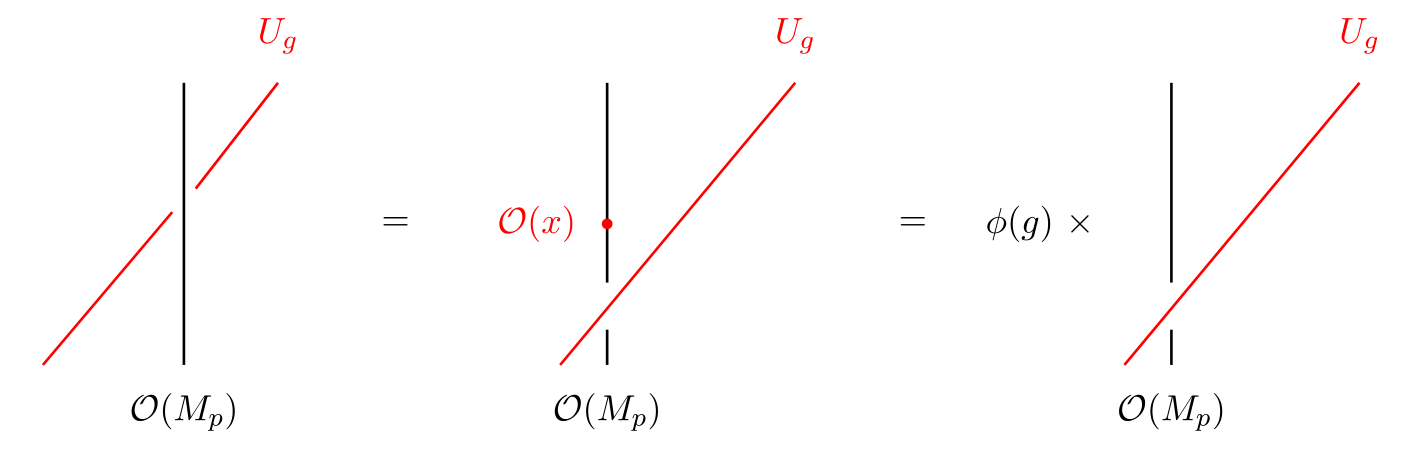
\includegraphics[scale=0.4]{figures/linking2.png}
	\caption{Taken from Bhardwaj}
\end{figure}
The composition of the group induces a composition of those functions $\phi(g)$, 
$$
\phi(g)\phi(g')=\phi(gg').
$$
Therefore the functions $\phi(g)$ form a 1-dimensional representation of the $p$-form group $G^p$.  Since $G^p$ is an abelian group, from Schur’s Lemma we know that every irreducible representation of this group is 1-dimensional, then the functions $\phi(g)$ form precisely the irreducible representation of the group $G^p$. Therefore, the operators $\mathcal{O}(M_p)$ transforms under the fundamental representations of the $p$-form group, which shows that the charged objects under $p$-form symmetries are extended operators supported on $p$-dimensional manifolds. 

We can easily generalize the result we have seen before for the Ward identity in terms of $p$-forms. For some  charged operator $\mathcal{O}(\Sigma_p)$ with charge $q\in\mathbb{Z}$ we have
$$
(d\star j)\mathcal{O}(\Sigma_D)=\delta^{D-p}(\Sigma_p)\mathcal{O}(\Sigma_D)
$$
where $\delta^{D-p}(\Sigma_p)$  is the Poincaré dual of the delta function defined on $\Sigma_D$.
\section*{Discrete Gauge Symmetries }
\end{document}
